
%Corps du document :
%\setlength{\parindent}{1cm}    

\section{Conception d'ensemble de l'architecture applicative}


\subsection{Cycles de vie des objets métiers}

Voici le diagramme d'état de l'objet ``Contact'' :

\begin {center}
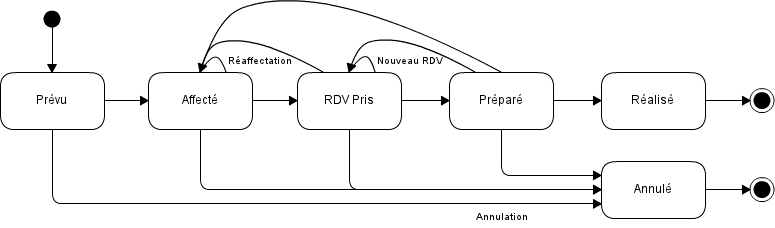
\includegraphics[width=\textwidth]{diagramme-etat-objet-contact.png}
\end {center}

\subsection{Choix de l'environnement technique}
L'environnement technique sera une architecture C/S 3-tiers :
\begin{itemize}
\item Couche de données : l'information est stockée ici sur la ou les bases de données. Ces informations seront récuperé par la couche applicative
\item Couche applicative : représente le coeur de l'architecture. A chaque demande de la couche de présentation, la couche applicative va effectuer un calcul et au besoin récuperer les informations de la base de données.
\item Couche de présentation : à chaque action de l'utilisateur, cette couche va transferer l'information à la couche applicative.
\end{itemize}
Le détail de ces tiers sera présenté dans le chapitre 'Architecture technique', notamment la localisation et la répartition des données.